\documentclass[conference]{IEEEtran}
\usepackage{graphicx}
\usepackage{amsmath}
\usepackage{cite}
\usepackage{url}

\title{A Modular Python Simulator for mmWave Vehicle-to-Infrastructure Link-Layer Research}

\author{\IEEEauthorblockN{mmWave V2I Simulator Contributors}
\IEEEauthorblockA{Open-source research simulator}}

\begin{document}
\maketitle

\begin{abstract}
We present an open-source Python simulator for mmWave vehicle-to-infrastructure (V2I) link-layer studies.
The tool replaces a prior MATLAB workflow with a modular, reproducible architecture supporting
synthetic and map-matched mobility, dual-band channel abstraction, runtime-selectable scheduling strategies,
and an interactive desktop GUI inspired by the original \texttt{vehicleBinPackSimulation.m} visualization.
The simulator targets researchers and practitioners who require license-free execution across macOS, Windows, and Linux.
\end{abstract}

\begin{IEEEkeywords}
mmWave, V2I, link-layer simulation, resource allocation, reproducible research
\end{IEEEkeywords}

\section{Introduction}
Millimeter-wave V2I systems require joint evaluation of mobility, blockage, beam alignment, and time-frequency resource allocation.
Prior MATLAB implementations demonstrated bin-packing-based allocation in urban vehicular scenarios but depend on licensed tooling and external executables.

This work provides a Python port with plugin interfaces for mobility, channel, scheduling, and visualization modules.

\section{Architecture}
The simulator is organized into deterministic core modules:
\begin{itemize}
  \item \textbf{Mobility}: synthetic lane-grid and CSV map-matched routes with city presets.
  \item \textbf{Channel}: geometric LOS/NLOS and dual-band (28/39 GHz) path-loss abstraction.
  \item \textbf{Scheduling}: pluggable strategies (Max-CQI, proportional fair, latency-aware).
  \item \textbf{GUI}: MATLAB-style map, packing panel, and trim-loss trend charts.
\end{itemize}

\section{Modeling Assumptions}
Channel behavior uses simplified 3GPP-inspired path loss and geometric blockage.
Scheduler/packing uses in-process Python algorithms rather than the original C++ rectangle-bin executable.
Validation compares density-sweep trim-loss trends against MATLAB-adjacent reference curves with documented caveats.

\section{Experiments}
We sweep vehicle counts $\{1,2,5,10,50\}$ and report mean trim loss and utilization.
Figure~\ref{fig:sweep} shows Python results against qualitative MATLAB-adjacent references.

\begin{figure}[t]
  \centering
  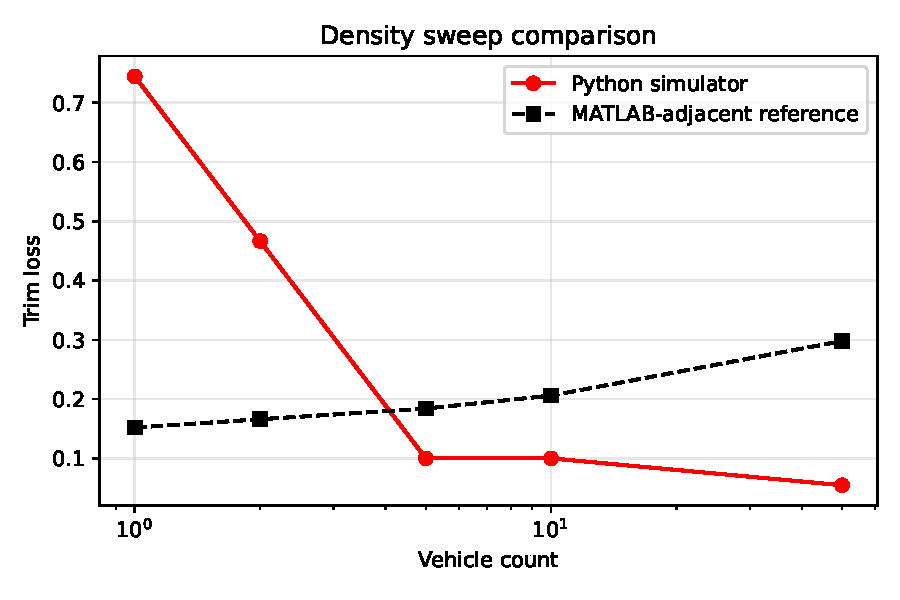
\includegraphics[width=\linewidth]{figures/fig_density_sweep.pdf}
  \caption{Vehicle-density sweep: trim loss comparison.}
  \label{fig:sweep}
\end{figure}

\begin{figure}[t]
  \centering
  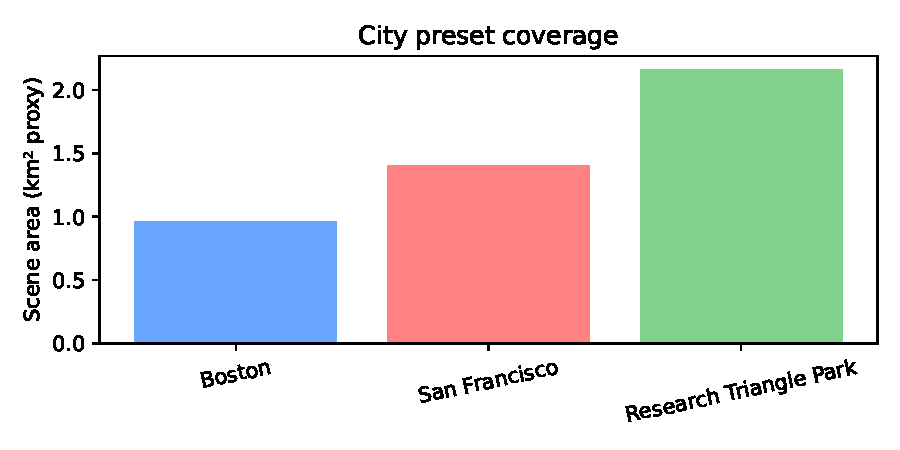
\includegraphics[width=0.48\linewidth]{figures/fig_city_presets.pdf}
  \hfill
  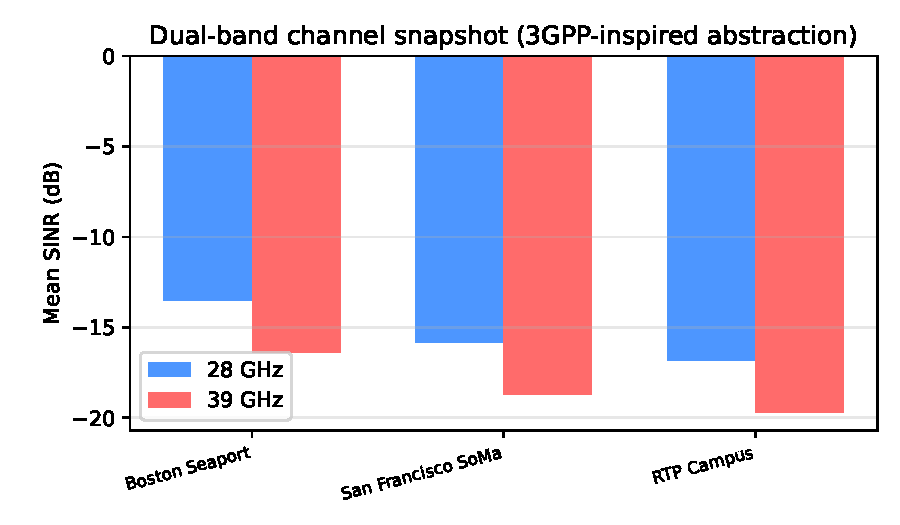
\includegraphics[width=0.48\linewidth]{figures/fig_dual_band.pdf}
  \caption{Left: open-license city preset extents. Right: mean dual-band SINR (28/39 GHz) across presets.}
  \label{fig:city_band}
\end{figure}

\section{Reproducibility}
Artifacts are generated via:
\texttt{python scripts/generate\_validation\_report.py} and
\texttt{bash scripts/build\_paper.sh}.
Fixed seeds yield deterministic JSON outputs.

\section{Conclusion}
The Python simulator provides a research-grade, extensible foundation for mmWave V2I link-layer experimentation without MATLAB licensing constraints.
The desktop release pairs MATLAB-style 2D visualization with ZIP session export; city presets and dual-band abstractions support comparative studies documented in the repository.

\section*{Acknowledgment}
This Python port is inspired by the original mmWave V2I MATLAB simulator (MathWorks File Exchange 84948).

\begin{thebibliography}{1}
\bibitem{subramanian2018}
R. Subramanian, ``A Resource Allocation Scheme for Multi-User MmWave Vehicle-to-Infrastructure Communication,'' \emph{Future Technologies Conference (FTC)}, 2018.
\bibitem{matlab84948}
R. Subramanian, ``Link Layer Simulator for mmWave V2I Network,'' MathWorks File Exchange, 2019.
\end{thebibliography}

\end{document}
